% !TeX root = ../My_thesis.tex
\chapter{АНАЛИЗ ЗАДАЧИ И ПРОЕКТИРОВАНИЕ ПРИЛОЖЕНИЯ} \label{ch1}

% не рекомендуется использовать отдельную section <<введение>> после лета 2020 года
%\section{Введение. Сложносоставное название первого параграфа первой главы для~демонстрации переноса слов в содержании} \label{ch1:intro}

% Хорошим стилем является наличие введения к главе, которое \textit{начинается непосредственно после названия главы, без оформления в виде отдельного параграфа}. Во введении может быть описана цель написания главы, а также приведена краткая структура главы. Например, в параграфе \ref{ch1:sec1} приведены примеры оформления одиночных формул, рисунков и таблицы. Параграф \ref{ch1:sec2} посвящён многострочным формулам и сложносоставным рисункам.

% Текст данной главы призван привести \textit{краткие} примеры оформления текстово-графических объектов. Более подробные примеры можно посмотреть в следующей главе, а также в рекомендациях студентам \cite{spbpu-student-thesis-template-author-guide}. 
Целью данной главы является описание задачи фильтрации IP-адресов по чёрному списку и обоснование принятых решений по структуре разрабатываемого программного продукта, организации ввода/вывода данных и реализуемому функционалу. В главе формулируются требования к проверке IP-адресов, описывается пользовательское взаимодействие с приложением (функционал меню, режимы работы) и приводятся основные сценарии использования (use cases) для интерактивной и пакетной проверки IP-адресов.

\section{Назначение и общая логика работы} \label{ch1:sec1}

Разработанное консольное приложение предназначено для проверки принадлежности IP-адреса к чёрному списку (blacklist) по заданным правилам фильтрации. Программа поддерживает два режима работы: (1) интерактивную проверку IP-адресов, вводимых с клавиатуры, и (2) пакетную проверку набора IP-адресов, загружаемого из JSON-файла, с формированием отчёта и рекомендациями по выбору алгоритма.
% Содержание первого подпараграфа первого параграфа первой главы.
Основная логика работы приложения:

\begin{itemize}
	\item Пользователь загружает чёрный список IP-адресов из JSON-файла
	\item Программа загружает данные в две структуры данных одновременно: HashSet и Bloom Filter
	\item Пользователь вводит IP-адрес для проверки или загружает файл со списком для проверки
	\item Программа проверяет IP-адрес обоими методами и сравнивает результаты
	\item Выводится результат проверки для каждого алгоритма отдельно
	\item Формируется статистика (память, время выполнения, вероятность ошибки для Bloom Filter)
	\item Генерируется рекомендация по выбору алгоритма для данного объёма данных
\end{itemize} 

Ключевое отличие алгоритмов:
\begin{itemize}
    \item HashSet — детерминированный алгоритм с 100\% точностью, но высоким потреблением памяти (хранит все элементы полностью)
    \item Bloom Filter — вероятностный алгоритм с возможностью False Positive (ложное срабатывание), но невозможностью False Negative (ложное отрицание), при этом значительно экономит память
\end{itemize}

\section{Назначение и общая логика работы} \label{ch1:sec2}

После запуска приложения пользователю отображается меню со следующими пунктами:

\begin{itemize}
	\item Загрузить blacklist из JSON - Пользователь вводит путь к JSON-файлу с чёрным списком IP-адресов. Программа загружает данные в обе структуры данных (HashSet и Bloom Filter) и подтверждает успешную загрузку.
	\item Проверить IP адрес — Пользователь вводит IP-адрес для проверки. Программа выполняет проверку обоими методами и выводит результат для каждого алгоритма отдельно (FOUND\/NOT\_FOUND).
	\item Сравнить алгоритмы — Программа выполняет проверку заранее заданного набора IP—адресов, выводит сравнительную статистику (память, время, вероятность ошибки) и формирует рекомендацию по выбору алгоритма.
	\item Справка — Приложение выводит краткую информацию о назначении программы и принципах работы алгоритмов фильтрации.
	\item Выход — Завершение работы приложения.
\end{itemize} 

Для более ясного понимания поведения программы приведем диаграмму случаев использования. Схема вкратце демонстрирует возможности пользователя, роль приложения относительно пользователя и как происходит взаимодействие с входными данными. ПО предоставляет пользователю гибкий интерфейс для работы с фильтрацией IP-адресов, позволяя как проверять отдельные адреса в интерактивном режиме, так и обрабатывать большие наборы данных в пакетном режиме с формированием детального отчёта.

\begin{figure}[ht!] 
	\center
	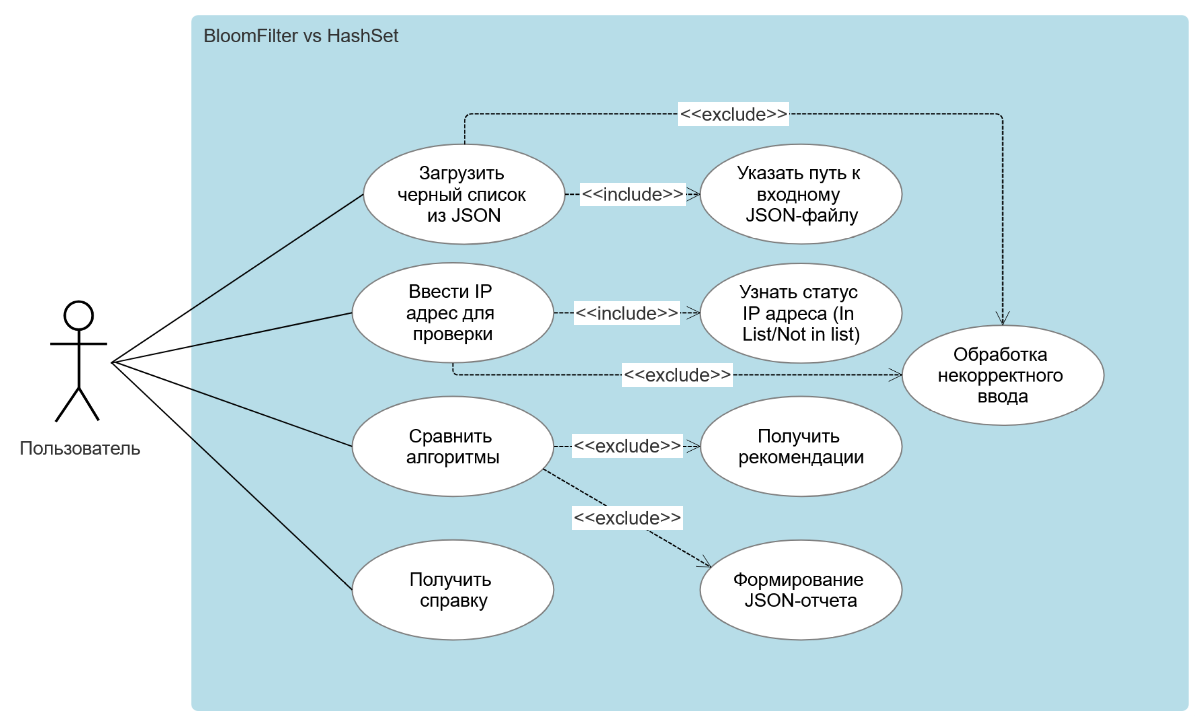
\includegraphics [scale=0.55] {my_folder/images/usecase.png}
	\caption{Диаграмма случаев-использования}  
\end{figure}


\section{Входные и выходные данные} \label{ch1:sec3}
Интерактивный режим принимает на вход путь к JSON-файлу с чёрным списком IP-адресов и отдельный IP-адрес для проверки (строка формата IPv4)
Пакетный режим принимает на вход JSON-файл произвольного размера, содержащий:
\begin{itemize}
	\item blacklist — массив IP-адресов для добавления в чёрный список
	\item checkIps — массив IP-адресов для проверки
\end{itemize} 

На выходе для интерактивного режима формируется статус проверки для каждого алгоритма (FOUND\/NOT\_FOUND) в консоль, тогда как для пакетного режима JSON-отчёт с полями: timestamp — время выполнения проверки, results — массив результатов для каждого IP, statistics — статистика, recommendation — текстовая рекомендация по выбору алгоритма.
% Одиночные формулы оформляют в окружении \texttt{equation}, например, как указано в следующей одиночной нумерованной формуле:
% %
%
% \begin{equation}% лучше не оставлять пропущенную строку (\par) перед окружениями для избежания лишних отсупов в pdf
% \label{eq:Pi-ch1} % eq - equations, далее название, ch поставлено для избежания дублирования
% \pi \approx 3,141.
% \end{equation}
%
%
% \begin{figure}[ht!] 
% 	\center
% 	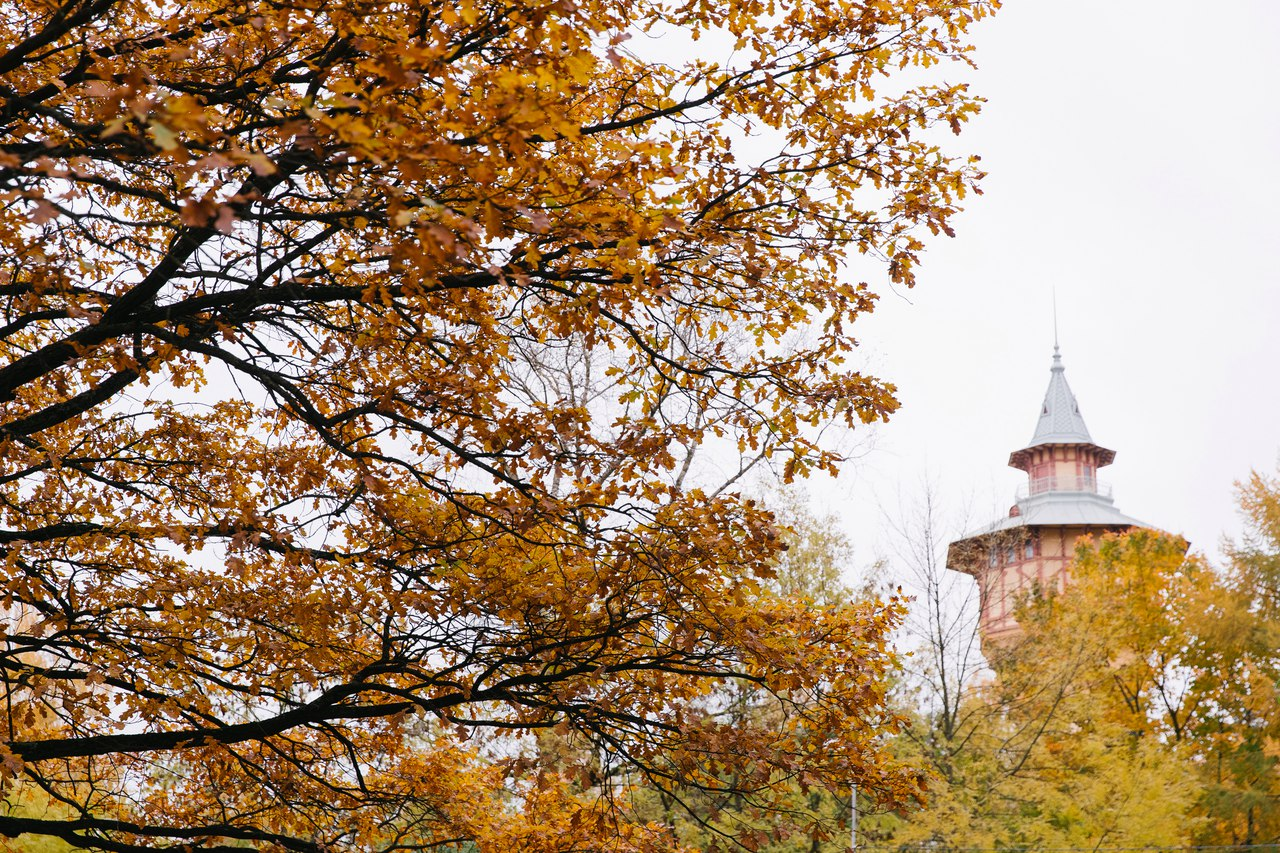
\includegraphics [scale=0.27] {my_folder/images//spbpu_hydrotower}
% 	\caption{Вид на гидробашню СПбПУ \cite{spbpu-gallery}} 
% 	\label{fig:spbpu_hydrotower}  
% \end{figure}
%
%
%\begin{table} [htbp]% Пример оформления таблицы
%	\centering\small
%	\caption{Представление данных для сквозного примера по ВКР \cite{Peskov2004}}%
%	\label{tab:ToyCompare}		
%		\begin{tabular}{|l|l|l|l|l|l|}
%			\hline
%			$G$&$m_1$&$m_2$&$m_3$&$m_4$&$K$\\
%			\hline
%			$g_1$&0&1&1&0&1\\ \hline
%			$g_2$&1&2&0&1&1\\ \hline
%			$g_3$&0&1&0&1&1\\ \hline
%			$g_4$&1&2&1&0&2\\ \hline
%			$g_5$&1&1&0&1&2\\ \hline
%			$g_6$&1&1&1&2&2\\ \hline		
%		\end{tabular}	
%	\normalsize% возвращаем шрифт к нормальному
%\end{table}


% \firef{} от figure reference
% \taref{} от table reference
% \eqref{} от equation reference

% На \firef{fig:spbpu_hydrotower} изображена гидробашня СПбПУ, а в \taref{tab:ToyCompare} приведены данные, на примере которых коротко и наглядно будет изложена суть ВКР.

\section{Проектирование программной структуры} \label{ch1:sec4}

Проектирование программной структуры приложения основано на принципах модульности и объектно-ориентированного подхода. В программе выделены несколько логически самостоятельных компонентов: модуль пользовательского интерфейса (консольное меню и ввод/вывод), модуль фильтрации IP-адресов (проверка принадлежности к чёрному списку), а также модуль ввода/вывода для пакетной обработки данных (загрузка пользователей из JSON и формирование отчёта).
Такой подход упрощает сопровождение и расширение программы: интерфейс взаимодействия с пользователем отделён от алгоритмов фильтрации, а работа с файлами и сериализацией вынесена в отдельный компонент.
Дополнительно модуль фильтрации реализован в виде набора интерфейсов и нескольких реализаций алгоритмов, что позволяет сравнивать подходы к проверке IP-адресов и использовать единый контракт при тестировании.

\subsection{Структура программы}

Для упрощения сопровождения и расширения программы логика приложения разделена на несколько модулей (пакетов) и классов:

\begin{itemize}
    \item Main. Точка входа в программу; инициирует запуск консольного приложения
    \item com.ipfilter.filter. Пакет, содержащий бизнес-логику фильтрации:
    \begin{itemize}
        \item IpFilter. Интерфейс для проверки IP-адресов
        \item HashSetIpFilter. Реализация алгоритма фильтрации на основе HashSet (детерминированный)
        \item BloomFilterIpFilter. Реализация алгоритма фильтрации на основе Bloom Filter (вероятностный)
    \end{itemize}
    \item com.ipfilter.service. Пакет для работы с сервисами:
    \begin{itemize}
        \item FilterService. Сервис обработки данных: загрузка blacklist, проверка IP, сравнение алгоритмов, формирование рекомендаций
        \item JsonHandler. Компонент обработки JSON: чтение входных данных и запись отчёта
    \end{itemize}
    \item com.ipfilter.model
    \begin{itemize}
        \item InputData. Модель входных данных (blacklist, checkIps)
        \item OutputData. Модель выходных данных (timestamp, results, statistics, recommendation)
        \item Модель результата проверки одного IP
        \item Модель статистики фильтрации (память, время, вероятность ошибки)
    \end{itemize}
\end{itemize}

Из преимуществ выбранной структуры можно выделить: азделение ответственности (каждый класс отвечает за одну задачу), тестируемость (интерфейсы позволяют использовать моки при тестировании), расширяемость (легко добавить новый алгоритм фильтрации, реализовав интерфейс IpFilter).

\newpage